\documentclass[11pt]{beamer}
% Compile with pdfLaTeX.

\usetheme{Boadilla}


\definecolor{SBred}{RGB}{153,0,0}
\definecolor{AttentionBlue}{RGB}{35,95,170}


\definecolor{SBred}{RGB}{153,0,0}
\definecolor{Ink}{RGB}{38,38,38}
\definecolor{Muted}{RGB}{105,105,105}

\makeatletter
\colorlet{beamer@blendedblue}{SBred}
\makeatother

\setbeamercolor{normal text}{fg=Ink,bg=white}
\setbeamercolor{frametitle}{fg=SBred,bg=white}
\setbeamercolor{structure}{fg=SBred}

% White footer text.
\setbeamercolor{author in head/foot}{fg=white,bg=SBred}
\setbeamercolor{title in head/foot}{fg=white,bg=SBred!70!white}
\setbeamercolor{date in head/foot}{fg=white,bg=SBred!45!white}

\setbeamerfont{frametitle}{size=\large}
\setbeamertemplate{navigation symbols}{}
\setbeamertemplate{page number in head/foot}[totalframenumber]
\setbeamersize{text margin left=7mm,text margin right=7mm}

\usepackage[T1]{fontenc}
\usepackage{lmodern,amsmath,amssymb,mathtools,booktabs,array,graphicx}
\usepackage{tikz}
\usetikzlibrary{positioning,arrows.meta,calc}

\hypersetup{
  colorlinks=true,
  urlcolor=SBred,
  pdftitle={Attention Factors for Statistical Arbitrage: Phase 1},
  pdfauthor={Jiaxi Cao}
}

\newcommand{\learn}[1]{\textcolor{SBred}{#1}}
\newcommand{\src}[1]{%
  \par\vfill
  {\fontsize{6.4}{7.6}\selectfont\color{Muted}#1\par}
}
\newcommand{\claim}[1]{%
  \par{\color{SBred}\bfseries #1\par}
}
\newcommand{\R}{\mathbb R}
\newcommand{\Var}{\operatorname{Var}}

\newcommand{\sbulogo}{%
  \IfFileExists{assets/sbu_logo.png}
    {
\includegraphics[width=22mm]{assets/sbu_logo.png}}
    {\textcolor{SBred}{\scriptsize Stony Brook University}}
}

% SBU logo at the upper right of each titled frame.
\setbeamertemplate{frametitle}{%
  \vspace{2mm}
  \begin{minipage}[c]{.75\textwidth}
    \raggedright\insertframetitle
  \end{minipage}\hfill
  \begin{minipage}[c]{.22\textwidth}
    \raggedleft\sbulogo
  \end{minipage}
  \vspace{2mm}
}

\title[Attention Factors]{%
  \textbf{Attention Factors for\\Statistical Arbitrage}
}
\subtitle{Phase I: literature, data and model}
\author[Jiaxi Cao]{Jiaxi Cao}
\institute[Stony Brook]{Stony Brook University}
\date[AMS 520]{%
  AMS 520: Machine Learning in Quantitative Finance\\Fall 2026
}

% Display the short title as plain text, without an internal link.
\makeatletter
\renewcommand{\insertshorttitle}[1][]{\beamer@shorttitle}
\makeatother

\newcommand{\threequestions}{%
  \[
  \boxed{\begin{array}{ccccc}
    \substack{\text{Which stocks}\\\text{are similar?}}
    &\longrightarrow&
    \substack{\text{What counts}\\\text{as mispricing?}}
    &\longrightarrow&
    \substack{\text{How to}\\\text{trade it?}}
  \end{array}}
  \]
}

\newcommand{\strategyroadmap}{%
  \[
  \boxed{\begin{array}{ccccc}
    \substack{\text{Which stocks}\\\text{are similar?}}
    &\longrightarrow&
    \substack{\text{What counts}\\\text{as mispricing?}}
    &\longrightarrow&
    \substack{\text{How to}\\\text{trade it?}}\\[4mm]
    \textcolor{SBred}{\text{Attention}}
    &&
    \textcolor{SBred}{\text{LongConv}}
    &&
    \textcolor{SBred}{\text{Net Sharpe + Explained Var.}}
  \end{array}}
  \]
}

\begin{document}
\begin{frame}{\phantom{Attention Factors for Statistical Arbitrage}}
\vspace{-4mm}\titlepage
\vspace{-5mm}
\begin{center}\scriptsize Based on Epstein, Wang, Choi and Pelger (ICAIF 2025)\\
\href{https://doi.org/10.1145/3768292.3770398}{doi:10.1145/3768292.3770398}\end{center}
\note{20 seconds. Today I will introduce Attention Factors for Statistical Arbitrage. I will begin with a pairs-trading example, then explain how attention builds comparison portfolios and how LongConv trades their residuals. I will finish with the joint objective, data requirements and Phase One findings.}
\end{frame}

\section{Statistical arbitrage and the comparison model}

\begin{frame}{Statistical Arbitrage: Pairs Trading}
Two similar firms move apart today: Hypothetically, $R_B = 2 R_A$.
\begin{center}
\begin{tabular}{@{}lrr@{}}\toprule
 & Firm A & Firm B\\\midrule
Today's return & $1\%$ & $3\%$\\
\textit{Hypothetical} return & $1\%$ & $2\%$\\\bottomrule
\end{tabular}
\end{center}
Buy the relative loser A; short the relative winner B.
\claim{Profit = The future relative move, after costs.}
\note{60 seconds. Pairs trading is a simple form of statistical arbitrage. Imagine two comparable firms. Today A rises one percent and B rises three percent. A is the relative loser, even though its price has increased. If we expect that difference to reverse, we could buy A and short B after today. Suppose tomorrow A rises three percent and B rises one percent. With half the gross exposure on each side, the trade earns one percent before costs. The profit comes from tomorrow's relative move. Today's separation does not guarantee a reversal; finding a reliable trading signal is part of the problem.}
\end{frame}

\begin{frame}{Building a Statistical Arbitrage Strategy}
\claim{Three Key Problems}
\threequestions
A naïve approach:
{\small\[
\text{Stocks}\longrightarrow\text{PCA factors}\longrightarrow
\text{Residuals}\longrightarrow\text{Find mean reversion}\longrightarrow\text{Trade}
\]}
But this does necessarily leads to profits.
\note{40 seconds. We have to answer three connected questions. Which stocks are similar? What counts as an unusual relative movement? And how should we trade it? A conventional route begins with stock returns, extracts PCA factors, computes residuals, looks for mean reversion, and then trades. PCA emphasizes explained historical variation. The later trading step must work with the comparisons that PCA has already chosen. This paper lets the trading objective influence those comparisons as well.}
\end{frame}

\begin{frame}{Joint Learning: The Paper's Roadmap}

\claim{Train the comparison portfolios and trading policy together.}
\strategyroadmap
\note{20 seconds. The central idea is to train the whole strategy together. Attention builds comparison portfolios. Their residual history enters LongConv, which produces trading positions. We then evaluate actual stock returns after costs through net Sharpe. Explained variance also anchors the factor model. These are parts of one joint fit.}
\end{frame}

\begin{frame}{The Factor Model}
\[
\underbrace{R_{i,t}}_{\text{stock return}}
=\underbrace{\beta_{i,t-1}^{\mathsf T}F_t}_{\text{common movement}}
+\underbrace{\epsilon_{i,t}}_{\text{idiosyncratic residual}}
\]
\begin{itemize}
\item $F_t$: factor returns, for example market, value, or momentum.
\item $\beta_{i,t-1}$: loadings, the response of the stock's return to each factor.
\item $\epsilon_{i,t}$: the idiosyncratic residue, commonly treated as firm-specific risk.
\end{itemize}
\note{45 seconds. The familiar factor model decomposes a stock's return. F contains factor returns, such as market, value or momentum. Beta contains the stock's loadings, or sensitivity to each factor. Beta transpose F adds up the common contributions. Epsilon is the remainder, commonly called the idiosyncratic residual or firm-specific risk. We can use this decomposition to explain price movements and to define deviations for statistical arbitrage. The equation works with returns, rather than an absolute dollar valuation.}
\end{frame}

\begin{frame}{Relative Deviations $\epsilon_{i,t}$}
By simple algebra,
\[
\epsilon_{i,t}=\underbrace{R_{i,t}}_{\text{actual return}}
-\underbrace{\beta_{i,t-1}^{\mathsf T}F_t}_{\text{factor-implied common return}}
\]
\begin{itemize}
\item A comparison basket supplies the relative benchmark.
\item We can measure deviation without estimating a fundamental dollar price.
\item Predictable future residual returns can support trading alpha.
\end{itemize}
\claim{Profit = The future relative move, after costs.}
\note{40 seconds. We can work directly with relative movements. Epsilon is actual return minus the factor-implied common return. The comparison basket supplies the benchmark, so we do not need to estimate the stock's fundamental dollar price first. If the stock returned one percent while its comparison returned two percent, its residual is minus one percent. The opportunity would come from predictable future residual returns. A negative residual alone does not establish that the stock is undervalued or that it will recover.}
\end{frame}



\begin{frame}{Attention Factors}

  \[
  \boxed{\begin{array}{ccccc}
    \substack{\textbf{Which stocks}\\\textbf{are similar?}}
    &\longrightarrow&
    \substack{\text{What counts}\\\text{as mispricing?}}
    &\longrightarrow&
    \substack{\text{How to}\\\text{trade it?}}\\[4mm]
    \textcolor{SBred}{\text{Attention}}
    &&
    \textcolor{SBred}{\text{LongConv}}
    &&
    \textcolor{SBred}{\text{Net Sharpe + Explained Var.}}
  \end{array}}
  \]
\end{frame}

\begin{frame}{Attention Identifies Similar Companies}
\begin{center}
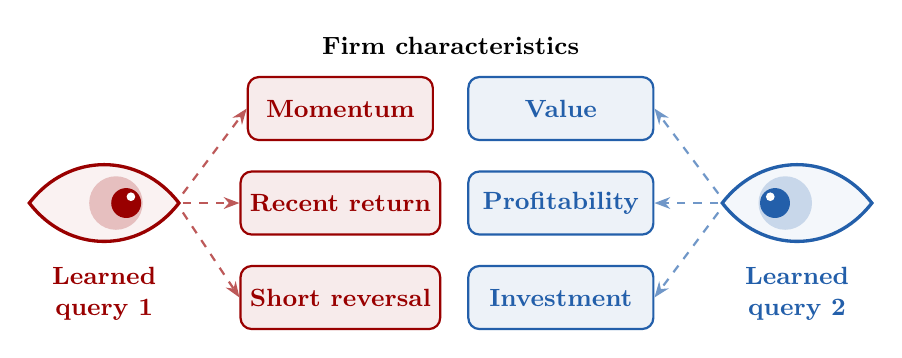
\begin{tikzpicture}[
  feature/.style={
    rounded corners=4pt,
    draw=gray!30,
    fill=gray!5,
    text=gray!65,
    minimum width=2.35cm,
    minimum height=8mm,
    font=\small
  },
  focus/.style={
    feature,
    draw=SBred,
    fill=SBred!8,
    text=SBred,
    font=\small\bfseries,
    thick
  },
  bluefocus/.style={
    feature,
    draw=AttentionBlue,
    fill=AttentionBlue!8,
    text=AttentionBlue,
    font=\small\bfseries,
    thick
  },
  gaze/.style={
    -{Stealth[length=2mm]},
    draw=SBred!65,
    thick,
    dashed
  },
  bluegaze/.style={
    -{Stealth[length=2mm]},
    draw=AttentionBlue!65,
    thick,
    dashed
  }
]

% Two illustrative groups emphasized by different learned queries.
\node[focus] (momentum) at (3.15,1.2) {Momentum};
\node[focus] (recent) at (3.15,0) {Recent return};
\node[focus] (reversal) at (3.15,-1.2) {Short reversal};

\node[bluefocus] (value) at (5.95,1.2) {Value};
\node[bluefocus] (profitability) at (5.95,0) {Profitability};
\node[bluefocus] (investment) at (5.95,-1.2) {Investment};

\node[font=\small\bfseries] at (4.55,2)
  {Firm characteristics};

% Red eye looking right.
\draw[draw=SBred,fill=SBred!5,line width=1.2pt]
  (-0.8,0)
  .. controls (-0.3,0.65) and (0.6,0.65) .. (1.1,0)
  .. controls (0.6,-0.65) and (-0.3,-0.65) .. cycle;

\fill[SBred!25] (0.3,0) circle (0.34);
\fill[SBred] (0.43,0) circle (0.19);
\fill[white] (0.49,0.08) circle (0.055);

\node[align=center,text=SBred,font=\small\bfseries]
  at (0.15,-1.15) {Learned\\query 1};

% Blue eye looking left.
\begin{scope}[shift={(9.1,0)},xscale=-1]
  \draw[draw=AttentionBlue,fill=AttentionBlue!5,line width=1.2pt]
    (-0.8,0)
    .. controls (-0.3,0.65) and (0.6,0.65) .. (1.1,0)
    .. controls (0.6,-0.65) and (-0.3,-0.65) .. cycle;

  \fill[AttentionBlue!25] (0.3,0) circle (0.34);
  \fill[AttentionBlue] (0.43,0) circle (0.19);
  \fill[white] (0.49,0.08) circle (0.055);
\end{scope}

\node[align=center,text=AttentionBlue,font=\small\bfseries]
  at (8.95,-1.15) {Learned\\query 2};

% Each eye attends to its matching group.
\draw[gaze] (1.15,0.12) -- (momentum.west);
\draw[gaze] (1.15,0) -- (recent.west);
\draw[gaze] (1.15,-0.12) -- (reversal.west);

\draw[bluegaze] (7.95,0.12) -- (value.east);
\draw[bluegaze] (7.95,0) -- (profitability.east);
\draw[bluegaze] (7.95,-0.12) -- (investment.east);

;

\end{tikzpicture}
\end{center}

\note{35 seconds. Attention provides a way to identify useful peers. We describe each firm through characteristics, then learn queries that select weighted baskets of firms. One query might emphasize technology companies, while another emphasizes banks. A company can participate in several baskets, so these are overlapping groups rather than hard sector assignments. The paper finds sector-like patterns even though industry labels are not supplied. We now look at the calculation that creates those baskets.}
\end{frame}



\begin{frame}{Attention Constructs Factor Basket}
\[
\underbrace{\widetilde X_{t-1}}_{N\times d}
=\underbrace{X_{t-1}}_{N\times M}\underbrace{\learn{W}}_{M\times d}
\]
\[
\underbrace{A_{t-1}}_{K\times N}
=\operatorname{softmax}_{\text{stocks}}\!\left(
\frac{
\underbrace{\learn{Q}}_{K\times d}
\underbrace{\widetilde X_{t-1}^{\mathsf T}}_{d\times N}
}{\sqrt d}\right)
\]
\begin{itemize}
\item The factor number $K$ and embedding dimension $d=32$ are separate settings.
\item Each row of $A$ is a factor basket with positive weights summing to one.
\item Dividing by $\sqrt{d}$ scales the attention scores to account for the embedding dimension.
\end{itemize}

\note{55 seconds. Let X contain one row of characteristics for each company. The learned matrix W K maps those rows into a shared key space. The superscript K is a label for the key projection, not a power and not a factor-count index. Next, each learned query scores the companies in that space. Softmax operates across stocks and converts the scores into portfolio weights. The factor count K says how many queries and baskets we want. The embedding width d says how many coordinates each key and query has. The paper uses thirty-two embedding coordinates. These two dimensions are separate.}
\end{frame}

\begin{frame}{Why keep a shared $W$?}
For example,
\[
X_i=(\text{momentum}_i,\text{size}_i,\text{value}_i,
     \text{profitability}_i,\text{volatility}_i,\ldots)
\]

\[
X_iW=\left(
0.7\,\text{momentum}_i
           -0.3\,\text{volatility}_i
\ldots,\ldots,\ldots
\right)
\]
\begin{itemize}
\item $W$ learns common combinations of the raw characteristics.
\item All factor queries compare firms in the same space.
\end{itemize}
\note{50 seconds. Why keep W K? It creates a common key space shared by every factor query. Raw inputs such as momentum, size, value, profitability and volatility can be mixed into learned coordinates. We might interpret some combinations as growth, defensiveness or value, but those names are only illustrations. The model learns numbers, not preassigned economic labels. Every query then asks a different question about the same coordinates. Mathematically, a linear projection can be absorbed into effective query coefficients; retaining W gives the architecture a shared representation whose width controls the parameterization.}
\end{frame}

\begin{frame}{An Example}
Take
\[
\frac{Q^K}{\sqrt{32}}=(1,0,\ldots,0)
\]
Then,
\begin{center}
\small
\begin{tabular}{@{}lcrr@{}}
\toprule
Firm & $\widetilde X_i$
     & $\dfrac{(Q^K)^{\mathsf T}\widetilde X_i}{\sqrt{32}}$
     & $A^K_{i}$\\
\midrule
NVDA & $(3.0,1.2,0,\ldots,0)$   & $3.0$  & $0.4078$\\
MSFT & $(2.7,1.0,0,\ldots,0)$   & $2.7$  & $0.3021$\\
AAPL & $(2.6,1.1,0,\ldots,0)$   & $2.6$  & $0.2734$\\
JPM  & $(-0.2,-0.8,0,\ldots,0)$ & $-0.2$ & $0.0166$\\
\bottomrule
\end{tabular}
\end{center}
\[
\frac{A^K_{\rm NVDA}}{A^K_{\rm JPM}}
=e^{3.0-(-0.2)}=e^{3.2}\approx24.5
\]
\note{60 seconds. Imagine thirty-two-coordinate keys, with the first two coordinates shown here and the rest zero. This illustrative scaled query selects the first coordinate. Its scores are three for Nvidia, two point seven for Microsoft, two point six for Apple, and minus point two for JPMorgan. These are hypothetical numbers. Softmax exponentiates the scores. Nvidia's weight divided by JPMorgan's weight is exponential three point two, or about twenty-four point five. The other firms affect their absolute weights, but not this ratio. Across five hundred firms, a query like this can create a technology-heavy basket. We repeat the calculation with different queries.}
\end{frame}

\begin{frame}{Sector Patterns Emerge}
Different factors emphasize technology, natural resources,
          finance and utilities

\begin{figure}
    \centering
    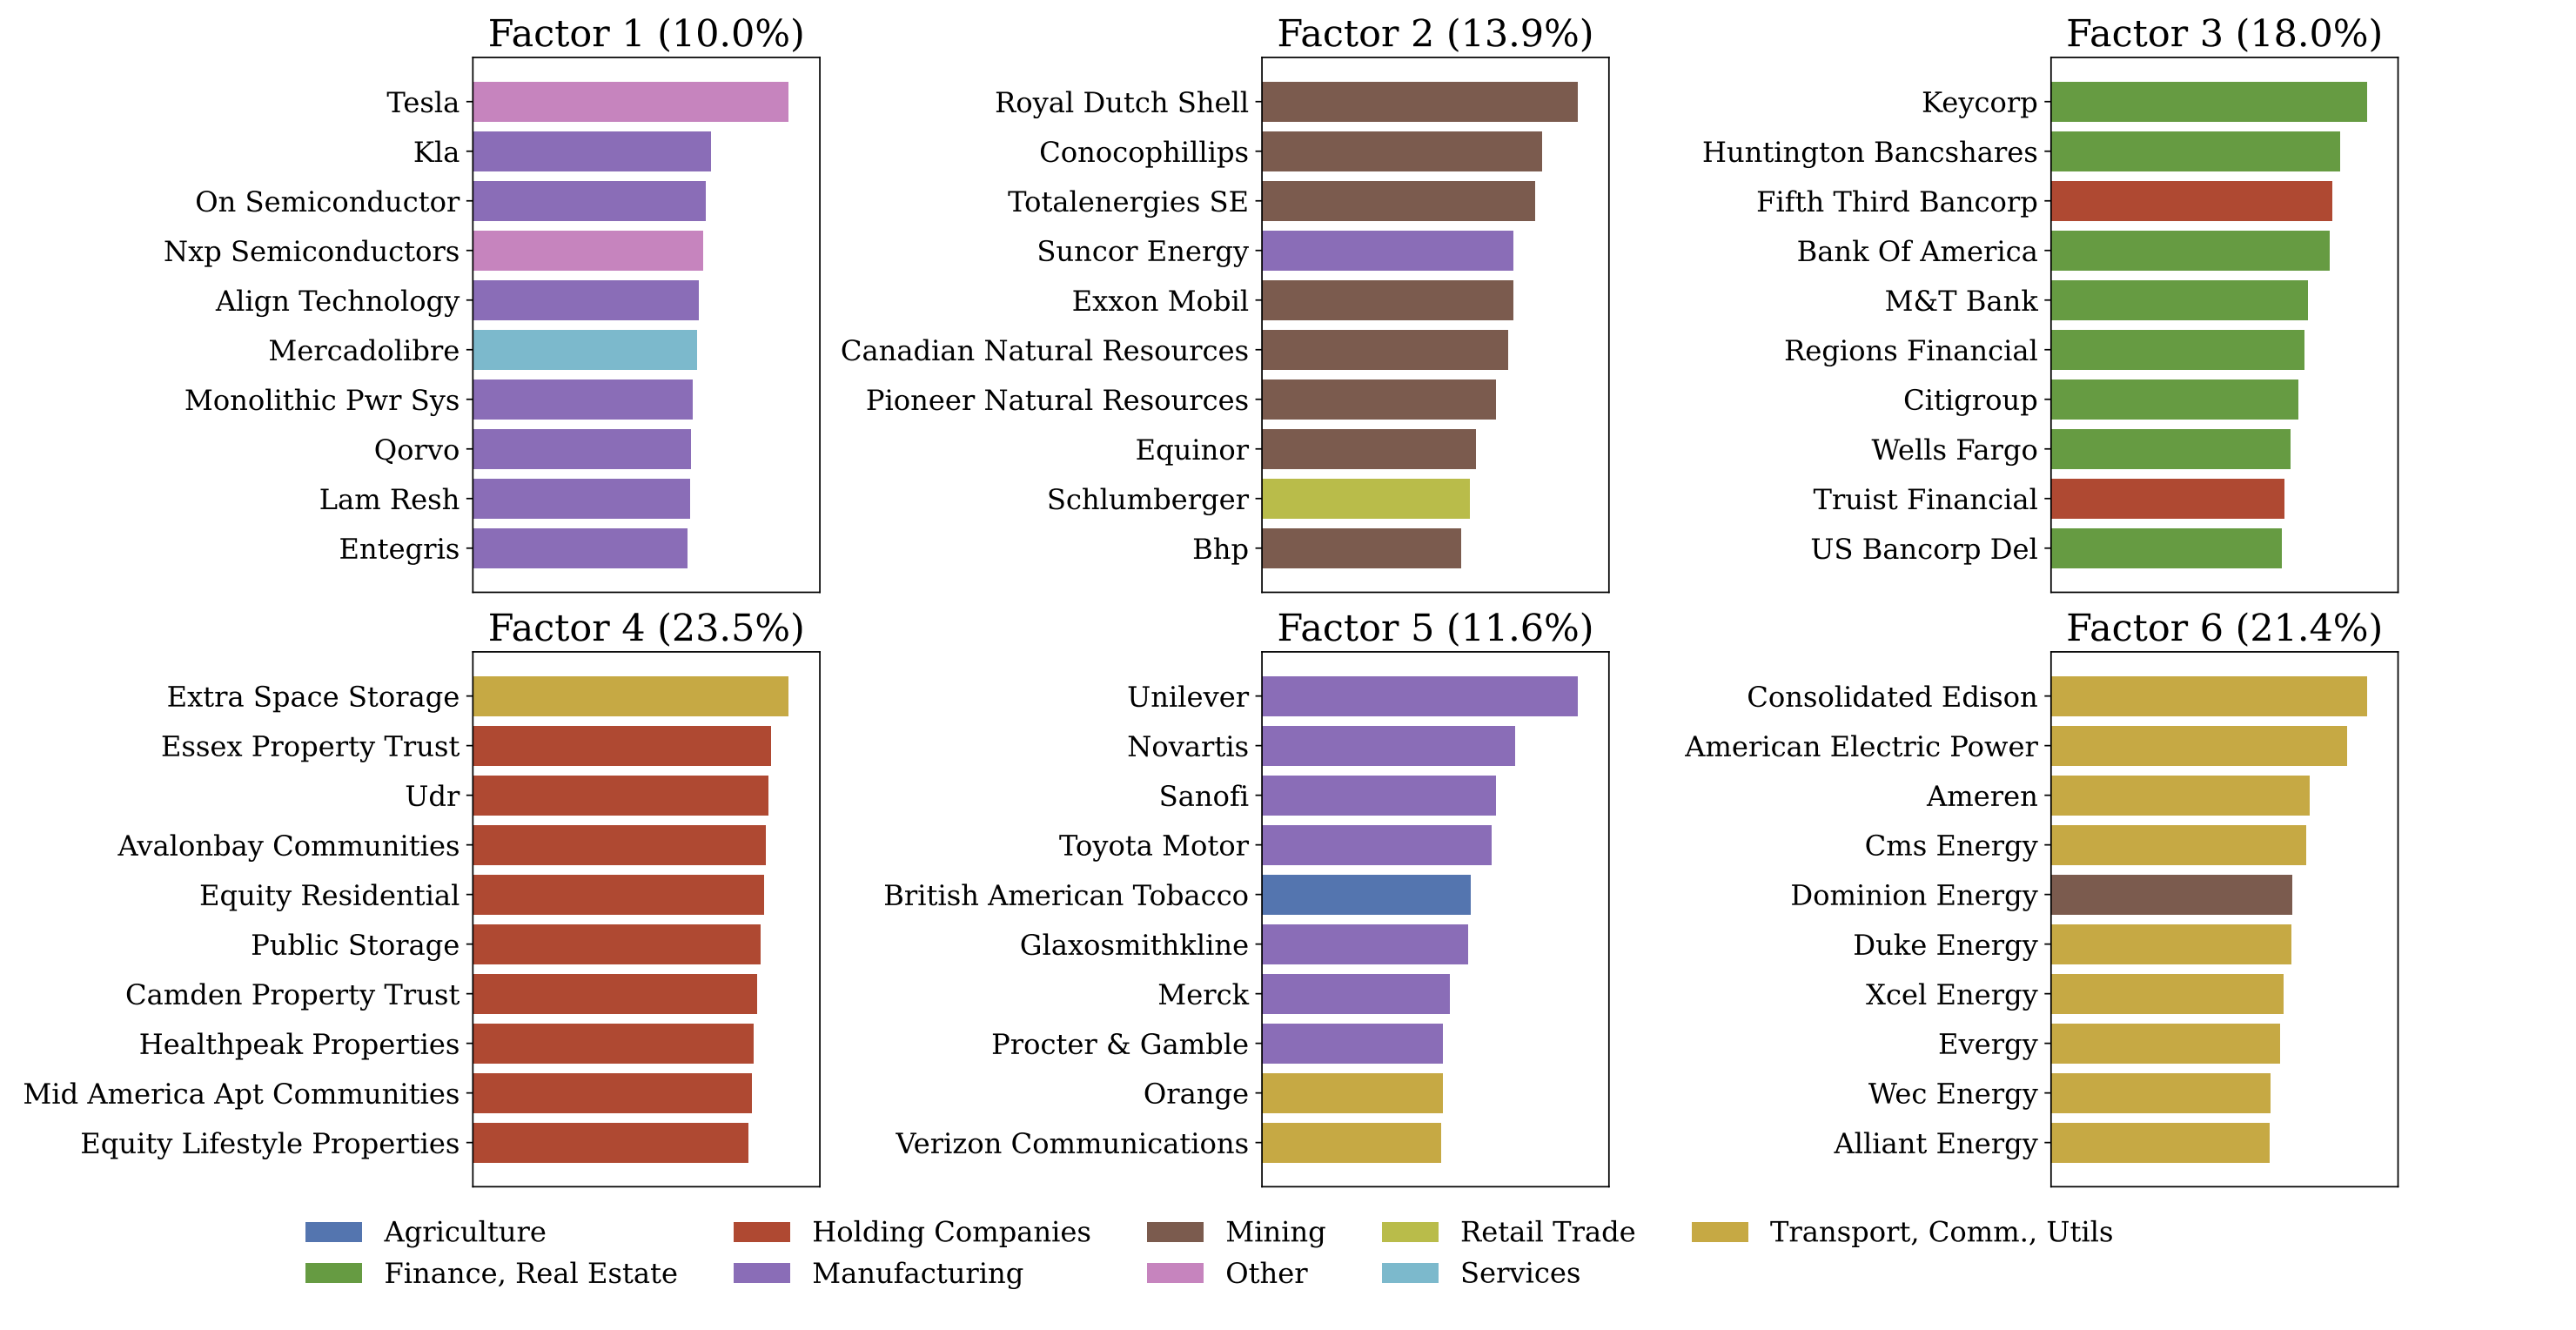
\includegraphics[
        width=\linewidth,
        height=4.0cm,
        keepaspectratio
    ]{assets/sector.png}
    \caption{Top 10 stocks in each of six attention-factor portfolios.}
    \label{fig:attention-sectors}
\end{figure}

\claim{Sector groups emerge without industry labels as inputs.}

\end{frame}

\begin{frame}{The Attention Matrix}
\[
A_{t-1}=\begin{bmatrix}
\text{weights from query }1\\
\text{weights from query }2\\
\vdots\\
\text{weights from query }K
\end{bmatrix}\in\R^{K\times N}
\]
\begin{itemize}
\item Rows correspond to factor baskets; Columns correspond to companies.
\item Each row sums to one.
\end{itemize}
\note{30 seconds. Stacking the query weights gives A, the attention matrix. Each column corresponds to a company and each row to a factor basket. If we choose thirty-two factors for an illustration, we get thirty-two queries and thirty-two rows. That choice is independent of having thirty-two key coordinates. The baskets can overlap. We now have portfolio weights; next we calculate the returns of those portfolios.}
\end{frame}

\begin{frame}{Factor Returns $F_t$}

Each row of $A$ defines a factor portfolio;
$F_t$ contains the realized factor returns.
\[
\underbrace{F_t}_{K\times1}
=\underbrace{A_{t-1}}_{K\times N}
\underbrace{R_t}_{N\times1}.
\]

The factor-implied stock returns are
$\widehat R_t=\beta_{t-1}^{\mathsf T}F_t$.
Substituting $F_t=A_{t-1}R_t$ gives
\[
\begin{aligned}
\epsilon_t
&=R_t-\beta_{t-1}^{\mathsf T}F_t\\[2mm]
&=\boxed{
\left(I_N-\beta_{t-1}^{\mathsf T}A_{t-1}\right)R_t
}.
\end{aligned}
\]

\claim{Choose loadings $\beta_{t-1}$ to minimize reconstruction error;
The residual $\epsilon_t$ measures deviation from factor-implied returns.}

\end{frame}


\begin{frame}{Loadings from Least-Squares Projection}


Write $A=A_{t-1}$ and $\beta=\beta_{t-1}$.
Project each column of $I_N^{\mathsf T}=I_N$ onto
$\operatorname{col}(A^{\mathsf T})$:
\[
I_N=A^{\mathsf T}\beta+E,
\qquad
\min_{\beta}\ \|E\|_F^2.
\]

Orthogonality gives the normal equations:
\[
AE=0
\quad\Rightarrow\quad
AA^{\mathsf T}\beta=A
\quad\Rightarrow\quad
\beta^{\mathsf T}=A^{\mathsf T}(AA^{\mathsf T})^{-1}.
\]

This inverse requires $AA^{\mathsf T}$ to be invertible,
so the factor baskets must be linearly independent.

\medskip
Add $\lambda_{\rm ridge}>0$ to ensure invertibility
and improve stability:
\[
\min_{\beta}\ \|I_N-A^{\mathsf T}\beta\|_F^2
+\lambda_{\rm ridge}\|\beta\|_F^2.
\]

\[
\boxed{
\beta_{t-1}^{\mathsf T}
=A^{\mathsf T}
\left(AA^{\mathsf T}+\lambda_{\rm ridge}I_K\right)^{-1}
}
\]

\end{frame}

\begin{frame}{The Residual Matrix}
\small

Residuals are relative-value portfolios: each stock is compared
with its factor-mimicking basket.
For stock $i$, row $i$ of $P$ gives the positions in that portfolio.

\[
\epsilon_t=R_t-\beta_{t-1}^{\mathsf T}F_t
=\underbrace{
\left(I_N-\beta_{t-1}^{\mathsf T}A_{t-1}\right)
}_{P_{t-1}}R_t.
\]

\[
\underbrace{P_{t-1}}_{500\times500}
=\underbrace{I_N}_{\text{own stock}}
-\underbrace{\beta_{t-1}^{\mathsf T}A_{t-1}}
            _{\text{factor-mimicking basket}}.
\]

\textbf{Example: NVDA versus its comparison basket}
\[
\begin{aligned}
\epsilon_{\mathrm{NVDA},t}\approx{}&
0.50R_{\mathrm{NVDA},t}\\
&-0.37R_{\mathrm{MSFT},t} -0.34R_{\mathrm{AAPL},t}+0.02R_{\mathrm{JPM},t}.
\end{aligned}
\]

\end{frame}

\begin{frame}{LongConv}

  \[
  \boxed{\begin{array}{ccccc}
    \substack{\text{Which stocks}\\\text{are similar?}}
    &\longrightarrow&
    \substack{\textbf{What counts}\\\textbf{as mispricing?}}
    &\longrightarrow&
    \substack{\text{How to}\\\text{trade it?}}\\[4mm]
    \textcolor{SBred}{\text{Attention}}
    &&
    \textcolor{SBred}{\text{LongConv}}
    &&
    \textcolor{SBred}{\text{Net Sharpe + Explained Var.}}
  \end{array}}
  \]
\end{frame}

\begin{frame}{LongConv: From History to a Position}
\[
\underbrace{(\epsilon_{i,t-30},\ldots,\epsilon_{i,t-1})}_{30\ \text{past residual returns}}
\quad\xrightarrow{\ \learn{\operatorname{LongConv}_\theta}\ }\quad
\underbrace{s_{i,t-1}}_{\text{residual position}}
\]
\begin{itemize}
\item $\theta$ are all trainable parameters in the LongConv.
\item LongConv is the paper's choice; A Transformer could replace it.
\item The same learned rule processes every residual portfolio.
\item A positive output takes the long side of that residual.
\end{itemize}
\claim{One decision uses residuals from past 30 days. Learning the rule uses eight years.}

\note{45 seconds. LongConv takes each residual portfolio's last thirty daily returns and produces a signed position. The same learned rule is shared across firms, and it can learn reversal or continuation patterns.

Thirty days is the information for one decision; eight years supplies the examples used to learn that rule. The temporal module is replaceable, for example by a Transformer. Its output is still a residual position, not a stock weight.}
\end{frame}

\begin{frame}{LongConv: Encode and Filter}

\claim{1. Encode each day's residual into 32 channels}\par
{
Input: $500\ \text{stocks}\times30\ \text{days}$;
$\tau=0,\ldots,29$ runs from the oldest day to yesterday.
\par}
\[
u_{i,h,\tau}
=\learn{a_h}\epsilon_{i,t-30+\tau}+\learn{b_h},
\qquad h=1,\ldots,32.
\]

\claim{2. Filter each channel through time}\par
{
Hidden tensors $u,y$:
$500\ \text{stocks}\times32\ \text{channels}\times30\ \text{days}$.
\par}
\[
y_{i,h,\tau}
=\underbrace{
\sum_{\ell=0}^{\tau}
\learn{\overline{\mathcal K}_{h,\ell}}u_{i,h,\tau-\ell}
}_{\text{weighted history}}
+\underbrace{
\learn{D_h}u_{i,h,\tau}
}_{\text{current-input skip}}.
\]

{Shrink small kernel weights:\par}
\[
\learn{\overline{\mathcal K}_{h,\ell}}
=\operatorname{sign}(\learn{\mathcal K_{h,\ell}})
\max\!\left(|\learn{\mathcal K_{h,\ell}}|-0.001,0\right).
\]


\end{frame}


\begin{frame}{LongConv: From Channels to a Position}

\claim{3. Combine final-day channels into one signed position}\par

Use the 32 channel outputs at the last known day ($\tau=29$).

\begin{center}
Input: $500\ \text{stocks}\times32\ \text{channels}$\\[1mm]
Output $s_{t-1}$: $500\ \text{residual positions}\times1$
\end{center}

\[
\boxed{
s_{i,t-1}
=\underbrace{\learn{b_s}}_{\text{bias}}
+\sum_{h=1}^{32}
\underbrace{\learn{v_h}}_{\text{channel weight}}\,
\underbrace{\phi(y_{i,h,29})}_{\text{fixed activation}}
}
\]

\[
\phi(x)=\max(x,0)\qquad\text{(ReLU)}.
\]

The learned bias $\learn{b_s}$ shifts the position.
A positive $s_{i,t-1}$ takes the long side of residual portfolio $i$;
a negative value takes the short side.

\end{frame}


\begin{frame}{Example: What Do Temporal Kernels Detect?}
\small

For illustration, set $\learn{a_h}=1$, $\learn{b_h}=0$,
and $\learn{D_h}=0$, so
$u_{i,h,\tau}=\epsilon_{i,t-30+\tau}$.
Kernel entries run from lag $0$ (yesterday) to lag $29$.

\medskip
\textbf{Channel 1: recent shock}
\[
\learn{\overline{\mathcal K}_1}=(1,0,\ldots,0)
\quad\Rightarrow\quad
y_{i,1,29}=\epsilon_{i,t-1}.
\]

\textbf{Channel 2: five-day average}
\[
\learn{\overline{\mathcal K}_2}
=\left(
\underbrace{\tfrac15,\ldots,\tfrac15}_{5\ \text{lags}},
0,\ldots,0
\right)
\quad\Rightarrow\quad
y_{i,2,29}
=\frac15\sum_{\ell=0}^{4}\epsilon_{i,t-1-\ell}.
\]

\textbf{Channel 3: day-to-day change}
\[
\learn{\overline{\mathcal K}_3}=(1,-1,0,\ldots,0)
\quad\Rightarrow\quad
y_{i,3,29}
=\epsilon_{i,t-1}-\epsilon_{i,t-2}.
\]

\end{frame}

\begin{frame}{Net Sharpe + Explained Variance}

  \[
  \boxed{\begin{array}{ccccc}
    \substack{\text{Which stocks}\\\text{are similar?}}
    &\longrightarrow&
    \substack{\text{What counts}\\\text{as mispricing?}}
    &\longrightarrow&
    \substack{\textbf{How to}\\\textbf{trade it?}}\\[4mm]
    \textcolor{SBred}{\text{Attention}}
    &&
    \textcolor{SBred}{\text{LongConv}}
    &&
    \textcolor{SBred}{\text{Net Sharpe + Explained Var.}}
  \end{array}}
  \]
\end{frame}

\begin{frame}{From Residual Positions to Stock Weights}

\claim{1. Combine the residual portfolios}\par
Each position $s_i$ scales row $i$ of $P$:
\[
\underbrace{\widetilde \omega_{t-1}}_{500\ \text{stocks}\times1}
=\underbrace{P_{t-1}^{\mathsf T}}_{500\times500}
\underbrace{s_{t-1}}_{500\ \text{residues}\times1}.
\]
Before normalization,
$$s_{t-1}^{\mathsf T}\epsilon_t
=s_{t-1}^{\mathsf T}P_{t-1}R_t
=\widetilde\omega_{t-1}^{\mathsf T}R_t.$$

\claim{2. Normalize total absolute exposure}\par
\[
\omega_{t-1}
=\frac{\widetilde \omega_{t-1}}{\|\widetilde \omega_{t-1}\|_1},
\qquad
\sum_j|\omega_{j,t-1}|=1.
\]

\end{frame}


\begin{frame}{From Stock Returns to Net Returns}
\small
\setlength{\abovedisplayskip}{2pt}
\setlength{\belowdisplayskip}{3pt}

Positions chosen at $t-1$ earn the stock returns $R_t$.

\claim{1. Compute the gross portfolio return}\par
\[
g_t=R_t^{\mathsf T}\omega_{t-1}.
\]

\claim{2. Charge stock trading and shorting costs}\par
\[
\mathrm{TO}_{t-1}
=\|w_{t-1}-w_{t-2}\|_1,
\qquad
(x)_+=\max(x,0).
\]
\[
c_{t-1}
=\underbrace{0.0005\,\mathrm{TO}_{t-1}}
            _{5\ \mathrm{bp}\ \text{per traded unit}}
+\underbrace{0.0001\sum_j(-w_{j,t-1})_+}
            _{1\ \mathrm{bp}\ \text{on short exposure}}.
\]

\claim{3. Subtract costs}\par
\[
n_t=g_t-c_{t-1}.
\]
\end{frame}


\begin{frame}{The Joint Training Objective}

Learn attention parameters $\learn{W^K},\learn{Q}$ and
LongConv parameters $\learn{\theta}$ together:
\[
\max_{\learn{W^K},\,\learn{Q},\,\learn{\theta}}
\left[
\underbrace{\frac{\overline n-R_f}{\sigma(n)}}
            _{\text{net Sharpe}}
+\lambda_{\rm Var}
\underbrace{
\frac1N\sum_{i=1}^{N}
\left(
1-\frac{\operatorname{Var}_t(\epsilon_{i,t})}
        {\operatorname{Var}_t(R_{i,t})}
\right)
}_{\text{explained variance}}
\right].
\]

\[
\overline n=\frac1T\sum_{t=1}^{T}n_t,
\qquad
\sigma(n)
=\sqrt{\frac1T\sum_{t=1}^{T}(n_t-\overline n)^2}.
\]

\begin{itemize}
\item Net Sharpe rewards risk-adjusted trading performance after costs.
\item Explained variance rewards a useful common-return representation.
\item The paper selects $\lambda_{\rm Var}=100$ using validation data.
\item Only the red parameters are learned during model training;
$\lambda_{\rm Var}$ is fixed after validation.
\end{itemize}

\end{frame}


\begin{frame}{Training and Results}

\textbf{Training and evaluation:}
\[
\text{8-year training window}
\quad\longrightarrow\quad
\text{Test out of sample the next year}
\]

\medskip
\textbf{Out-of-sample results:}
\begin{figure}
    \centering
    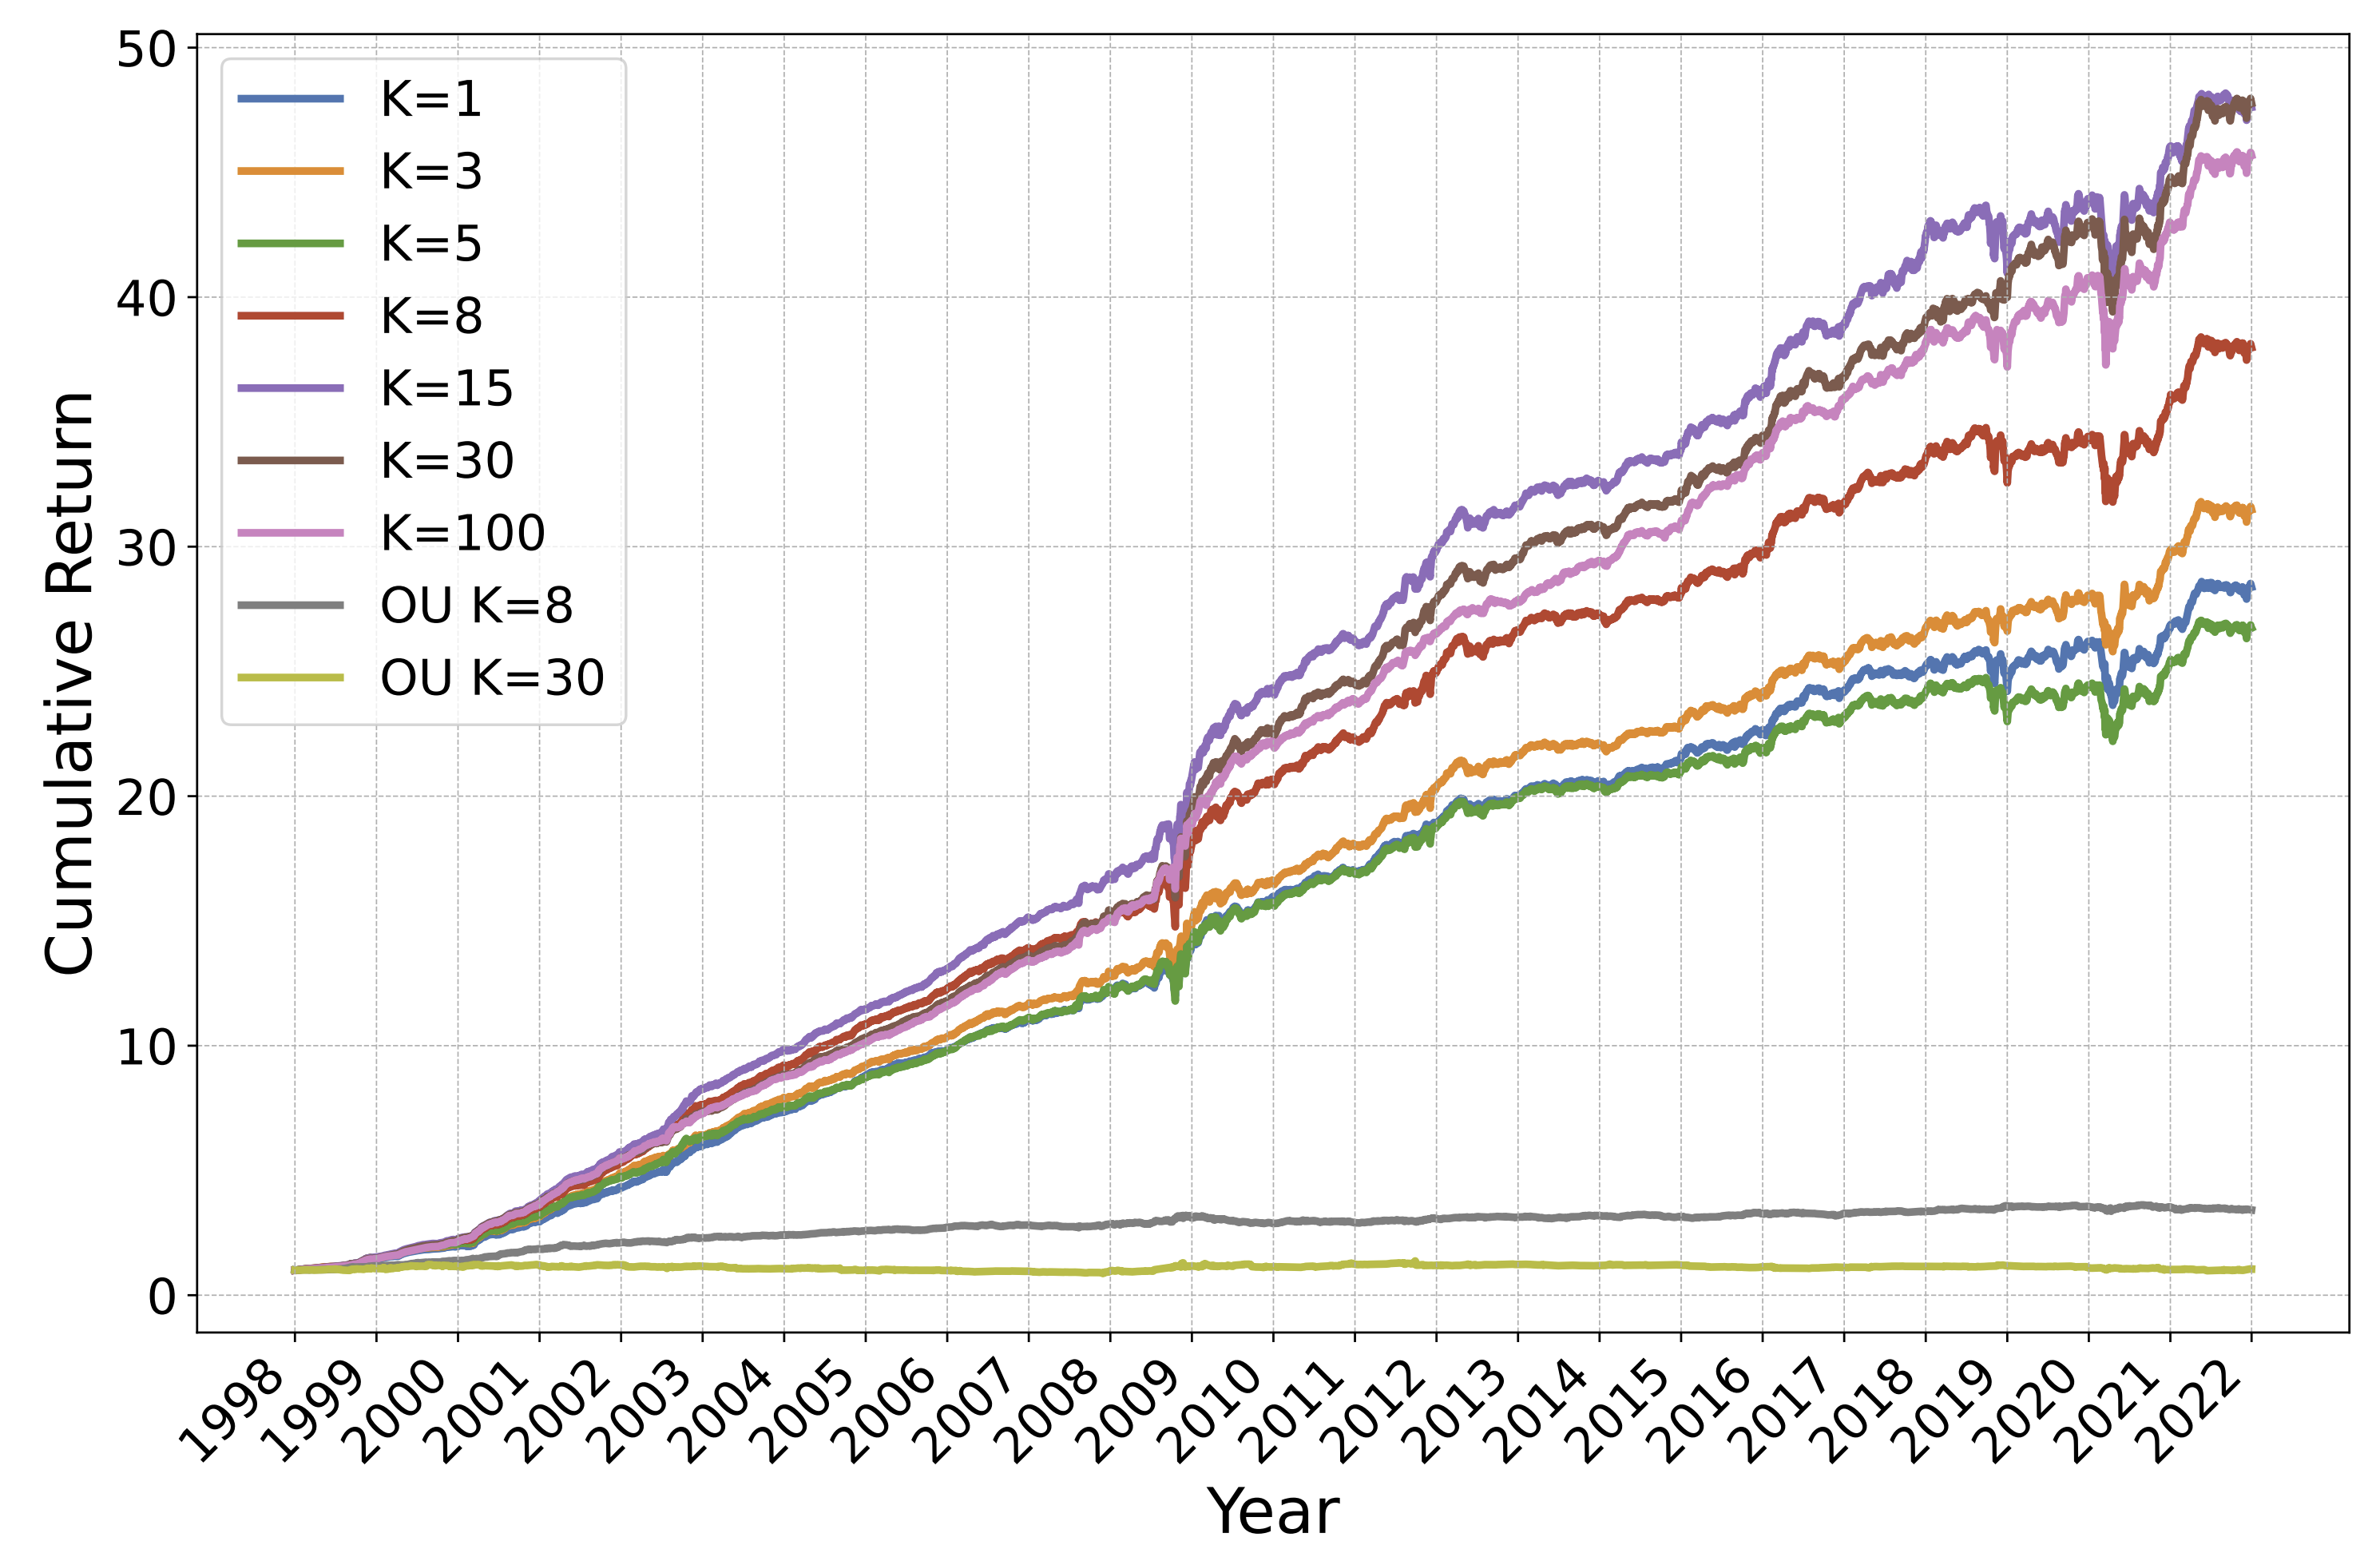
\includegraphics[
        width=.95\linewidth,
        height=4.0cm,
        keepaspectratio
    ]{assets/results.png}
    \caption{Cumulative out-of-sample returns:
    attention portfolios versus PCA + OU benchmarks,
    January 1998--December 2021.}
    \label{fig:attention-results}
\end{figure}

\end{frame}

\begin{frame}{Results}

\begin{center}
{\fontsize{6.4}{7.4}\selectfont
\setlength{\tabcolsep}{1.6pt}
\renewcommand{\arraystretch}{.90}

\begin{tabular}{@{}lrrrrrrrr@{}}
\toprule
Model & $K$ & SR & $\mu$ & $\sigma$
& $\mathrm{SR}_{\rm net}$ & $\mu_{\rm net}$
& $\sigma_{\rm net}$ & Beta\\
\midrule
Attention & 1 & 3.05 & 14.45 & 4.74 & 1.68 & 7.94 & 4.72 & 0.05\\
 & 3 & 3.05 & 14.91 & 4.89 & 1.69 & 8.25 & 4.87 & 0.06\\
 & 5 & 2.92 & 14.21 & 4.87 & 1.58 & 7.66 & 4.85 & 0.07\\
 & 8 & 3.35 & 15.70 & 4.68 & 1.94 & 9.05 & 4.66 & 0.07\\
 & 15 & 3.81 & 16.66 & 4.37 & 2.25 & 9.78 & 4.35 & 0.06\\
 & \textbf{30} & \textbf{3.97} & \textbf{16.66}
 & \textbf{4.20} & \textbf{2.28} & \textbf{9.52}
 & \textbf{4.18} & \textbf{0.05}\\
 & 100 & 4.52 & 16.45 & 3.64 & 2.19 & 7.93 & 3.62 & 0.05\\
\midrule
PCA + OU & 1 & 0.40 & 1.85 & 4.57 & -2.54 & -11.62 & 4.57 & 0.02\\
 & 3 & 1.26 & 4.18 & 3.33 & -2.72 & -9.04 & 3.33 & 0.01\\
 & 5 & 0.99 & 2.91 & 2.93 & -3.44 & -10.11 & 2.93 & 0.00\\
 & 8 & 0.78 & 2.04 & 2.61 & -4.15 & -10.83 & 2.61 & 0.00\\
 & 10 & 0.80 & 1.99 & 2.50 & -4.32 & -10.80 & 2.50 & 0.00\\
 & 15 & 0.51 & 1.12 & 2.20 & -5.24 & -11.53 & 2.20 & 0.00\\
 & 30 & 0.18 & 0.40 & 2.24 & -6.45 & -14.74 & 2.29 & -0.00\\
 & 100 & -0.35 & -0.66 & 1.87 & -7.05 & -13.23 & 1.88 & -0.00\\
\midrule
PCA + LongConv & 1 & 2.26 & 13.10 & 5.79 & 1.19 & 6.98 & 5.78 & 0.10\\
 & 3 & 2.76 & 14.61 & 5.30 & 1.57 & 8.29 & 5.28 & 0.07\\
 & 5 & 2.41 & 14.10 & 5.86 & 1.30 & 7.62 & 5.84 & 0.10\\
 & 8 & 2.64 & 14.88 & 5.63 & 1.50 & 8.42 & 5.61 & 0.09\\
 & 10 & 2.66 & 14.94 & 5.61 & 1.52 & 8.48 & 5.59 & 0.09\\
 & 15 & 2.56 & 14.74 & 5.75 & 1.41 & 8.08 & 5.73 & 0.09\\
 & 30 & 2.79 & 15.15 & 5.42 & 1.57 & 8.47 & 5.40 & 0.09\\
 & 100 & 2.66 & 14.36 & 5.40 & 1.44 & 7.75 & 5.38 & 0.09\\
\midrule
Market & -- & 0.42 & 8.61 & 20.37 & 0.42 & 8.61 & 20.37 & 1.00\\
\bottomrule
\end{tabular}
\par}
\end{center}

{\scriptsize
Out-of-sample annualized performance, January 1998--December 2021.
\par}

\note{50 seconds. Table Two reports all the paper's model configurations
and distinguishes gross from net performance. The thirty-factor attention
model has a gross annualized Sharpe of 3.97 and a net annualized Sharpe
of 2.28. Its net annual return is 9.52 percent. At the same factor count,
PCA with LongConv achieves a net Sharpe of 1.57, while PCA with the
parametric OU threshold rule has a net Sharpe of minus 6.45.
This comparison shows why performance after costs matters.
Increasing attention to one hundred factors raises the gross Sharpe
to 4.52, but lowers net Sharpe to 2.19. The highest gross Sharpe
therefore does not deliver the highest net Sharpe among the reported
configurations. The beta column measures exposure to the market,
not the stock-to-factor loadings discussed earlier.}

\end{frame}



\begin{frame}{The 79 Model Inputs}

For each stock, we combine characteristic ranks with their raw
cross-sectional medians and the risk-free rate:
\[
\underbrace{39\ \text{rank quantiles}}
            _{\text{vary across firms}}
+\underbrace{39\ \text{raw medians}}
             _{\text{common at a date}}
+\underbrace{1\ \text{risk-free rate}}
            _{\text{common at a date}}
=79.
\]

\begin{center}
\begin{tabular}{@{}lrlr@{}}
\toprule
Characteristic group & Count & Characteristic group & Count\\
\midrule
Past returns & 8 & Trading frictions & 10\\
Value & 8 & Profitability & 7\\
Investment & 3 & Intangibles & 3\\
\bottomrule
\end{tabular}
\end{center}

At each date, the model input matrix is
\[
\underbrace{X_{t-1}}_{500\ \text{stocks}\times79\ \text{inputs}}
\in\mathbb R^{500\times79}.
\]
\end{frame}

\begin{frame}{Example: Ranks and Medians}
\small

At one date, rank five firms by size (market capitalization).
An illustrative normalization is
\[
q_i=\frac{\operatorname{rank}(x_i)-1}{5-1}.
\]

\begin{center}
\begin{tabular}{@{}lrrr@{}}
\toprule
Firm & Raw size (\$bn) & Rank & Rank quantile $q_i$\\
\midrule
A & $10$   & $1$ & $0.00$\\
B & $20$   & $2$ & $0.25$\\
C & $30$   & $3$ & $0.50$\\
D & $40$   & $4$ & $0.75$\\
E & $1000$ & $5$ & $1.00$\\
\bottomrule
\end{tabular}
\end{center}

\textbf{Median:} the middle value after sorting, here $30$ billion.
This raw median is added to every firm's inputs at this date.

\textbf{Purpose of rank quantiles:}
Put characteristics on a common scale and preserve relative order;
the extreme size $1000$ becomes the bounded rank $1.00$.

\textbf{The raw median retains level information that ranks lose.}

\end{frame}


\begin{frame}{Future Goals}
\begin{itemize}
    \item Test the model on the latest data.
    \item Use reinforcement learning or online optimization
          to review current holdings, aiming to reduce
          trading costs and improve net Sharpe.
\end{itemize}
\end{frame}


\begin{frame}{References}
\scriptsize
\begin{itemize}
\item Epstein, Wang, Choi and Pelger (2025). \emph{Attention Factors for Statistical Arbitrage}. \href{https://doi.org/10.1145/3768292.3770398}{ICAIF paper}.
\item Avellaneda and Lee (2010). \emph{Statistical Arbitrage in the US Equities Market}.
\item Guijarro-Ordonez, Pelger and Zanotti. \emph{Deep Learning Statistical Arbitrage}. \href{https://arxiv.org/abs/2106.04028}{Author manuscript}.
\item Chen, Pelger and Zhu. \emph{Deep Learning in Asset Pricing}. \href{https://arxiv.org/abs/1904.00745}{Author manuscript and Internet Appendix}.
\item Fu et al. (2023). \emph{Simple Hardware-Efficient Long Convolutions for Sequence Modeling}. \href{https://proceedings.mlr.press/v202/fu23a.html}{ICML}.
\item WRDS, CRSP and Compustat primary documentation. Local Try1 source and methodology audits.
\end{itemize}
\note{The target paper is the authority for this model and its published results. The earlier statistical-arbitrage papers provide the literature context, and the asset-pricing appendix provides delegated characteristic definitions. The original LongConv paper explains the sequence method; its reference implementation does not establish the finance paper's exact wrapper. WRDS, CRSP, and Compustat documentation support the raw-data construction. Our report keeps these sources separate from local implementation choices and Try1 audit findings.}
\end{frame}




\begin{frame}{Thanks!}
\claim{Any questions?} 
\end{frame}




\begin{frame}{Published training settings}
\small
\begin{tabular}{@{}lr@{}}\toprule
Setting & Paper value\\\midrule
Attention embedding & 32\\
LongConv hidden channels / layers & 32 / 1\\
Residual lookback & 30 trading days\\
Training window / refit & 8 years / annual\\
Epochs / learning rate & 30 / 0.003\\
Optimizer named in text & Adam\\
Dropout / LongConv weight decay & 0.1 / 0.05\\
Explained-variance coefficient & 100\\
Kernel squash threshold & 0.001\\
Factor counts & $1,3,5,8,10,15,30,100$\\\bottomrule
\end{tabular}\par
\note{This table collects the settings actually stated in the paper. Attention has thirty-two embedding coordinates. LongConv has one layer, thirty-two channels, and a thirty-day residual lookback. The model uses an eight-year window, annual retraining, thirty epochs, and a learning rate of point zero zero three. Dropout is point one, LongConv weight decay is point zero five, and explained variance receives weight one hundred. The text names Adam, although its citation points to AdamW, so the optimizer interpretation needs to be recorded.}
\end{frame}




\begin{frame}{Unpublished implementation choices}
\small
\begin{tabular}{@{}>{\raggedright\arraybackslash}p{.36\textwidth}>{\raggedright\arraybackslash}p{.56\textwidth}@{}}\toprule
Item & Recorded Try1 choice / limitation\\\midrule
Ridge & $10^{-6}$ from initial validation\\[1mm]
Seeds & 0, 1, 2; paper gives no count or values\\[1mm]
Encoder/readout & Linear encoder, GELU, dropout, last-step linear readout\\[1mm]
Initialization & Standard linear initialization, normal queries and skip\\[1mm]
Training objective schedule & One complete eight-year objective update per epoch\\[1mm]
Memory chunks & Original FP32 schedule: 256 days\\[1mm]
Ranks, missing histories & Declared cohort/tie/range rules and explicit coverage flags\\\bottomrule
\end{tabular}\par
\note{This table separates our choices from published settings. Try1 selected a ridge of ten to the minus six using the initial validation period and used seeds zero, one, and two. It records a particular encoder and readout, initialization rules, and one full-window update per epoch. The original float-thirty-two run uses two-hundred-and-fifty-six-day memory chunks. These choices were not selected to match test-period results. A later K-thirty continuation has its own recorded protocol and must be distinguished from that original run.}
\end{frame}


\begin{frame}{Past-return characteristics: 8}
\small
\begin{tabular}{@{}l>{\raggedright\arraybackslash}p{.68\textwidth}@{}}\toprule
Name & Definition / source\\\midrule
\texttt{r2\_1} & Previous month's RET\\
\texttt{r12\_2} & Compound monthly RET, months $m-12$ to $m-2$\\
\texttt{r12\_7} & Compound RET, $m-12$ to $m-7$\\
\texttt{r36\_13} & Compound RET, $m-36$ to $m-13$\\
\texttt{ST\_Rev} & Previous month's RET, duplicate under reference definition\\
\texttt{Ret\_D1} & Previous session's daily RET\\
\texttt{Ret\_W1} & Previous-week compound RET\\
\texttt{STD\_W1} & Previous-week daily-return SD\\\bottomrule
\end{tabular}\par
\note{These eight inputs summarize different parts of the return history. The monthly momentum variables cover different lag ranges; for example, r twelve two compounds months twelve through two before the current month. The short-term momentum and reversal rows both use the prior month under the reference definition, so we retain that duplicate rather than silently remove it. The final three rows use the previous day or week. Try1 defines a week as five trading sessions and records a sample-standard-deviation choice for weekly volatility.}
\end{frame}

\begin{frame}{Value characteristics: 8}
\small
\begin{tabular}{@{}l>{\raggedright\arraybackslash}p{.73\textwidth}@{}}\toprule
Name & Computed annual formula\\\midrule
\texttt{A2ME} & AT / December market equity\\
\texttt{BEME} & Derived book equity / December market equity\\
\texttt{C} & CHE / AT\\
\texttt{CF} & (NI + DP - WCAPCH - CAPX) / book equity\\
\texttt{CF2P} & (IB + DP + TXDB) / December market equity\\
\texttt{Q} & (AT + ME - CEQ - TXDB) / AT\\
\texttt{Lev} & (DLTT + DLC) / (DLTT + DLC + SEQ)\\
\texttt{E2P} & IB / December market equity\\\bottomrule
\end{tabular}\par
\note{Most of these value inputs are computed ratios, rather than fields downloaded directly. Assets, earnings, and cash flow are compared with market equity or book equity. Book equity itself requires a documented construction from accounting fields, and the market-equity denominators use the specified December date. Two details deserve attention. The literal cash-flow formula needs WCAPCH, which is absent from our modern retained records. The Q definition also has a prose-versus-field inconsistency, so we record the literal fields used instead of silently replacing them.}
\end{frame}

\begin{frame}{Investment characteristics: 3}
\small
\begin{tabular}{@{}l>{\raggedright\arraybackslash}p{.72\textwidth}@{}}\toprule
Name & Computed annual formula\\\midrule
\texttt{Investment} & $(AT-AT^{-})/AT^{-}$\\[3mm]
\texttt{NOA} & $NOA^{\$}/AT^{-}$\\[3mm]
\texttt{DPI2A} & $\{\Delta PPEGT+\Delta INVT\}/AT^{-}$\\\bottomrule
\end{tabular}\par
\vspace{4mm}
\[
\begin{aligned}
NOA^{\$}={}&(AT-CHE-IVAO)\\
&-(AT-DLC-DLTT-MIB-PSTK-CEQ).
\end{aligned}
\]
\note{These inputs require adjacent annual statements. Investment measures asset growth relative to prior-year assets. Net operating assets subtract operating liabilities from operating assets and scale the result by prior-year assets. DPI-two-A measures changes in gross property, plant, equipment, and inventory, again relative to prior assets. The minus superscript means the adjacent prior fiscal year. We need both valid inputs and the correct availability date before a new annual value can enter a trading decision.}
\end{frame}

\begin{frame}{Trading-friction characteristics: 10}
\scriptsize
\begin{tabular}{@{}l>{\raggedright\arraybackslash}p{.71\textwidth}@{}}\toprule
Name & Direct level or computed statistic\\\midrule
\texttt{AT} & Annual total assets, Compustat AT\\
\texttt{LME} & Previous month market equity, CRSP PRC and SHROUT\\
\texttt{LTurnover} & Previous month's share volume / shares outstanding\\
\texttt{Rel2High} & Adjusted month-end price / prior 12-month high\\
\texttt{Resid\_Var} & Prior two months' FF3 daily excess-return residual variance\\
\texttt{Spread} & Prior-month mean of $(ASK-BID)/\{(ASK+BID)/2\}$\\
\texttt{SUV} & Prior-month unexplained volume relative to 60-session fit\\
\texttt{Variance} & Prior two calendar months' daily return variance\\
\texttt{Vol} & Previous-week daily volume sum\\
\texttt{Beta} & 5-year 3-day log-excess correlation times 1-year SD ratio\\\bottomrule
\end{tabular}\par
\note{This group mixes direct levels with calculated market statistics. Assets is an accounting level, while size and share turnover use CRSP data. The price-to-high variable needs adjusted prices. Residual variance uses a past Fama-French regression, and spread uses closing bid and ask quotes rather than daily high and low. Unexplained volume requires a historical regression. The final beta uses a correlation and volatility-ratio construction, rather than simply one ordinary regression coefficient. Every window and missing-data rule is documented in the report.}
\end{frame}

\begin{frame}{Profitability characteristics: 7}
\small
\begin{tabular}{@{}l>{\raggedright\arraybackslash}p{.73\textwidth}@{}}\toprule
Name & Computed annual formula\\\midrule
\texttt{PROF} & (SALE - COGS) / derived book equity\\
\texttt{CTO} & SALE / $AT^{-}$\\
\texttt{FC2Y} & (chosen XSGA + XRD + XAD) / SALE\\
\texttt{OP} & (REVT - COGS - XSGA - interest) / book equity\\
\texttt{PM} & OIADP / SALE\\
\texttt{RNA} & OIADP / $NOA^{\$,-}$\\
\texttt{D2A} & DP / AT\\\bottomrule
\end{tabular}\par
\note{These measures compare operating quantities with assets, sales, or book equity. PROF uses sales less cost of goods sold, while capital turnover uses sales over prior assets. Fixed costs combine selling and administrative expenses, research and development, and advertising. Missing expenses are not automatically zero. Operating profitability also needs an interest-expense choice because the reference has a field inconsistency. The remaining measures use operating income or depreciation. We calculate a raw ratio only when its required components and denominator are valid.}
\end{frame}

\begin{frame}{Intangible characteristics: 3}
\small
\begin{tabular}{@{}l>{\raggedright\arraybackslash}p{.74\textwidth}@{}}\toprule
Name & Computed annual formula\\\midrule
\texttt{OA} & $[\Delta ACT-\Delta CHE-\Delta LCT-\Delta DLC-\Delta TXP-DP]/AT^{-}$\\[3mm]
\texttt{OL} & (COGS + XSGA) / AT\\[3mm]
\texttt{PCM} & (SALE - COGS) / SALE\\\bottomrule
\end{tabular}\par
\vspace{3mm}\small The OA signs follow the cited appendix literally. They differ from the conventional working-capital accrual formula.
\note{The category label comes from the paper's characteristic table. Operating accruals uses annual changes in several balance-sheet fields and depreciation. The signs shown follow the delegated appendix literally, even though they differ from a common working-capital accrual formula. Operating leverage is cost of goods sold plus selling and administrative expenses over assets. Price-cost margin is sales less cost of goods sold, divided by sales. These are annual computed inputs, so their public availability still needs a reporting lag.}
\end{frame}


\end{document}
